% !TEX root = ../main.tex
\section{Results}
\label{sec:results}

The results answer four questions in sequence: whether comparison metrics can grade (no), why (their variance belongs to the reference), when they can still rank models (when references are worth predicting), and what does grade (verification).
Each answer below leads with its finding, and every number joins the canonical analysis of Section~\ref{sec:setup}.

\subsection{RQ1: Can reference-similarity metrics grade individual solutions? No.}
\label{sec:classnull}

No comparison metric grades individual solutions against blind human soundness.
On the 60-item random label set, the five comparison metrics correlate with human soundness at $-0.16$ $[-0.46, +0.13]$ (\tfa), $-0.27$ $[-0.54, +0.04]$ (gold-token log-probability; $n{=}42$, the subset with logprob available), $-0.08$ $[-0.33, +0.18]$ (TF-IDF), $-0.33$ $[-0.58, -0.12]$ (unigram-F1), and $+0.14$ $[-0.08, +0.40]$ (embeddings); Figure~\ref{fig:class} plots the full field, and the full class table is Appendix~\ref{app:classtable}.
Every interval includes zero except unigram-F1's, which is weakly negative.
On the same solutions the LLM judge reaches \judgetbd, and the single-point prefix-repair signal at $k{=}0.5$ reaches $+0.76$.

Code replicates the null against an oracle no one can argue with.
On 492 freshly generated solutions scored by executing the official test suites, \tfa's correlation with passing is $0.00$, and stays within $[-0.04, +0.06]$ inside each model.
(This is the per-solution correlation; the model-level code ranking is Table~\ref{tab:map}'s $+0.43$ row.)
The soft log-probability version does no better.

\begin{figure}[t]
\centering
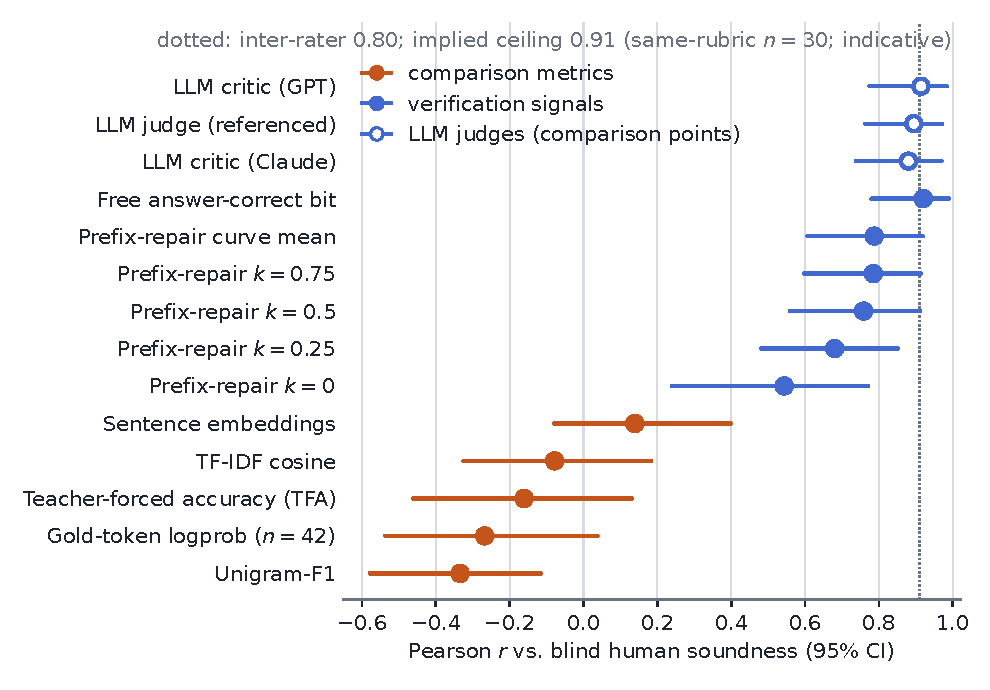
\includegraphics[width=0.92\textwidth]{figures/fig_class.pdf}
\caption{\textbf{The class-level null on the 60-item random label set.}
Pearson correlation with blind human soundness, with bootstrap 95\% CIs, for every signal in the canonical analysis: comparison metrics in orange, verification signals in blue, and LLM judges (expensive comparison points) as hollow markers.
\textbf{Takeaway:} every comparison metric straddles zero while every verification signal grades, and the prefix-repair curve mean sits at the human inter-rater ceiling of $0.79$.}
\label{fig:class}
\end{figure}

\subsection{RQ2: Why not? Comparison scores are reference properties.}
\label{sec:mechanism}

Most of a comparison score's per-solution variance is a property of the reference, not of the solution.
We decomposed per-solution \tfa{} across a grid of fifteen to sixteen models from four families (the count varies by benchmark with model availability), after removing each model's overall level.
Between $83\%$ and $92\%$ of the remaining variance is an \emph{item main effect}: a component identical across families.
Such a component can only be a property of the reference, namely how predictable this particular gold text is.
Another $3$--$7\%$ is family-specific style, and this style channel roughly doubles on saturated benchmarks (\textsc{GSM8K} $7.2\%$, full \textsc{MATH} $6.5\%$, versus \textsc{Putnam} $2.9\%$).
The same structure appears in code ($78\%$ item, $8\%$ family, $14\%$ residual), and attenuated in every similarity metric (item share: log-probability $83$--$91\%$, embeddings ${\sim}70\%$, TF-IDF $69\%$).

The item effect has a name: reference perplexity.
Across 6{,}000 model--item pairs on \textsc{MATH-500}, \tfa{} correlates with the reference's bits-per-character under the same model at $r = -0.895$ (Figure~\ref{fig:mechanism}), so reference perplexity explains $80\%$ of the pooled variance.
This is a different accounting from the $83$--$92\%$ item share above: the decomposition splits variance across models and items, while this pools everything, and both point the same way.
To first order, teacher-forced accuracy measures how compressible the reference is.
A score that is four-fifths about the reference cannot grade the solution in front of it.

An intervention on the references confirms the mechanism causally.
Across benchmarks, the model-ranking signal of Section~\ref{sec:ranking} correlates $+0.89$ with mean reference entropy and $-0.81$ with saturation, but the two are confounded in observational data.
So we intervened: on the same \textsc{MATH-500} items, replacing each worked reference with the single line ``The final answer is [answer]'' collapses the ranking signal from $+0.35$ to $+0.02$.
Predicting a long, information-dense reference requires skill adjacent to solving the problem.
Predicting a formulaic one requires nothing, leaving only style.

\begin{figure}[t]
\centering
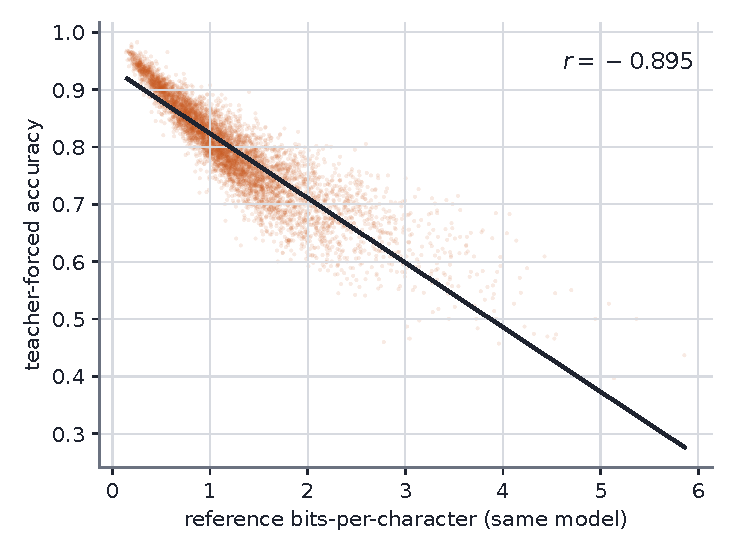
\includegraphics[width=0.62\textwidth]{figures/fig_mechanism.pdf}
\caption{\textbf{Teacher-forced accuracy is reference perplexity.}
Per-solution \tfa{} against the reference's bits-per-character under the same model, pooled over 6{,}000 model--item pairs on \textsc{MATH-500}, with the least-squares fit.
\textbf{Takeaway:} at $r = -0.895$, reference compressibility explains $80\%$ of pooled \tfa{} variance, so \tfa{} meters the reference rather than grading the solution.}
\label{fig:mechanism}
\end{figure}

\subsection{RQ3: When can matching rank models? When references are worth predicting.}
\label{sec:ranking}

Averaged over a benchmark, mean \tfa{} ranks models by accuracy on hard data and not at all on easy data.
Every family ladder is positive on the three olympiad benchmarks (twelve of twelve family--benchmark cells), while on the easiest benchmarks five of twelve family ladders invert.
Table~\ref{tab:map} shows the full boundary: the pooled cross-family correlation runs from $\rho = +0.86$ on olympiad math down through zero and into reversal on saturated data.

\begin{table}[t]
\centering
\small
\setlength{\tabcolsep}{2.5pt}
\begin{tabular}{llcc}
\toprule
benchmark & regime & cross-family $\rho$ [95\% CI] & within-family $\rho$ \\
\midrule
\textsc{Omni-MATH} & olympiad & $\mathbf{+0.86}$ $[+0.35, +1.00]$ & $+0.90$ \\
\textsc{Putnam-AXIOM} & olympiad & $+0.60$ $[+0.17, +0.83]$ & $\mathbf{+1.00}$ \\
\textsc{Putnam-Variations} & olympiad, contamination-proof & $+0.38$ $[-0.15, +0.73]$ & $+0.90$ \\
\textsc{HumanEval} & code & $+0.43$ $[-0.02, +0.76]$ & $+0.80$ \\
\textsc{MATH-500} & competition math & $+0.35$ $[-0.15, +0.71]$ & $+0.90$ \\
\textsc{MATH} (full) & competition math, near-saturated & $+0.21$ $[-0.29, +0.61]$ & $+0.60$ \\
\textsc{GSM8K} & grade school, saturated & $-0.25$ $[-0.71, +0.33]$ & $+0.70$ \\
\textsc{GSM8K-Platinum} & grade school, relabeled & $-0.19$ $[-0.71, +0.41]$ & $+0.60$ \\
\textsc{SWE-bench Verified} & agentic code & $0.00$ (8 coder models) & $\mathbf{+1.00}$ (Qwen-Coder) \\
\bottomrule
\end{tabular}
\caption{\textbf{The boundary map: where reference matching ranks models.}
Cross-family Spearman correlation between mean \tfa{} and accuracy (17 models; bootstrap CIs), and the Qwen size-ladder correlation as the within-family column, per benchmark; best values in bold.
Ranking degrades from olympiad to saturated benchmarks, with code sitting mid-scale, and within-family ladders survive everywhere the pooled comparison does not, because family style cancels inside a family and survives across families.
\textbf{Takeaway:} matching ranks models only on hard benchmarks with information-dense references, and cross-family comparison needs a shared style or a verifier.}
\label{tab:map}
\end{table}

The positive side of the boundary is worth stating as plainly as the negative.
Comparison metrics do rank models, under three conditions that all hold at once:
\begin{enumerate}
\item \textbf{Use them in aggregate, never per item.}
The reference-predictability nuisance is identical for every model on a given item, so it cancels when scores are averaged over a benchmark; per-item it dominates.
\item \textbf{The reference must be detailed enough to be worth predicting.}
A long worked solution differentiates strong models from weak ones; an answer line does not (the $+0.35 \to +0.02$ intervention of Section~\ref{sec:mechanism}).
\item \textbf{The benchmark must be hard enough to differentiate models.}
On saturated data every model predicts the reference about equally well, and the leftover variance is writing style, which is why saturated rankings collapse or invert.
\end{enumerate}

The agentic setting obeys the same boundary.
On \textsc{SWE-bench Verified}, patch-level \tfa{} ranks the four Qwen-Coder sizes perfectly ($\rho = +1.00$) yet carries no cross-family signal ($\rho = 0.00$, eight models).
Family style survives averaging, so cross-family comparison needs a shared style or a verifier.
The consequence for leaderboards: reference matching is legitimate exactly when these conditions hold, and reference entropy can be measured in advance to check the second one.

\paragraph{Repairs fail as predicted: the class is empty, not under-tuned.}
\label{sec:slate}
No reweighting rescues the per-solution metric, and the mechanism predicted every failure in advance.
A natural response to RQ1 is that some reweighting rescues the metric; the mechanism predicts otherwise, and we tested that prediction adversarially.
Every variant in Table~\ref{tab:slate} was proposed either by our reviewers or by the mechanism itself, and the directional outcome was registered in the repository before the run.

\begin{table}[t]
\centering
\footnotesize
\setlength{\tabcolsep}{2pt}
\begin{tabular}{llll}
\toprule
proposed metric & class & registered prediction & outcome \\
\midrule
position-weighted \tfa{} (late tokens up-weighted) & comparison & null & decays $+0.13 \to -0.37$ \\
entropy-normalized \tfa{} (perplexity residualized) & comparison & null & ranking $+0.13 \to -0.17$ \\
seven reweightings (IDF, surprisal, masking, \dots) & comparison & null & all $\le 0$ \\
answer-swap counterfactual & verification & works & $+$ in 8/9 models, mean $+0.13$ \\
prefix-repair curve & verification & works & $\mathbf{+0.79}$ vs.\ human soundness \\
\bottomrule
\end{tabular}
\caption{\textbf{The taxonomy makes correct advance predictions.}
All four pre-registered predictions landed as called (the seven reweighting variants predate the registration protocol and are included for completeness); the strongest judge-free signal is in bold.
The two verification-class entries are described in Section~\ref{sec:verify}.
\textbf{Takeaway:} every comparison-class repair failed and every verification-class signal worked, exactly as registered before the data existed.}
\label{tab:slate}
\end{table}

The position-weighting sweep shows the intuitive repair making the metric monotonically worse.
On \textsc{GSM8K}-style data one might weight early reference tokens less than the final ones.
With weights $w \propto (\mathrm{pos}/n)^{\gamma}$ over per-token hit vectors for twelve cross-family models on \textsc{MATH-500} (a subset of the map's seventeen; its pooled baseline is $+0.13$ rather than $+0.35$ because five models lack per-token data), ranking holds at $+0.13$ through $\gamma{=}1$, reaches zero by $\gamma \in [4,8]$, and hits $-0.37$ when only the last four tokens count (Figure~\ref{fig:sweeps}, left).
The repair converges to the answer-only-reference null of Section~\ref{sec:mechanism} and then overshoots it, because the variance being redistributed is reference nuisance rather than soundness.

Entropy normalization is the complementary test, and it empties the metric.
Residualizing bits-per-character out of \tfa{} removes the one thing it robustly measures, and nothing is left: ranking falls from $+0.13$ to $-0.17$, and the item-level signal is null both raw ($-0.11$) and partialed ($+0.09$).

\begin{figure}[t]
\centering
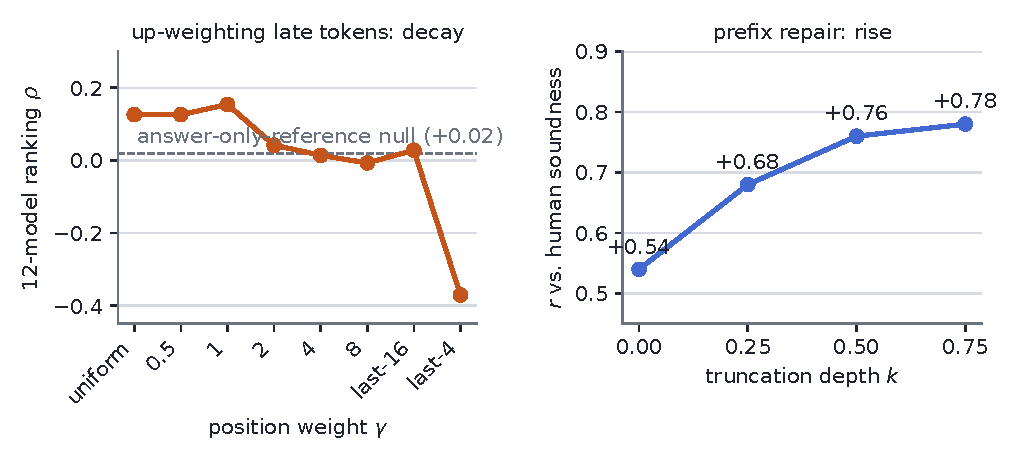
\includegraphics[width=0.95\textwidth]{figures/fig_sweeps.pdf}
\caption{\textbf{The two registered sweeps move in opposite directions, as the taxonomy predicts.}
Left: up-weighting late reference tokens (the intuitive repair) decays \tfa's twelve-model ranking signal monotonically past $\gamma{=}1$, through the answer-only-reference null and beyond it.
Right: the prefix-repair signal rises monotonically with truncation depth, from a pure difficulty probe ($k{=}0$) to $+0.78$ against human soundness at $k{=}0.75$, with a curve mean of $+0.79$.
\textbf{Takeaway:} repairing a comparison metric destroys it while deepening a verification signal strengthens it, which is the class divide made visible.}
\label{fig:sweeps}
\end{figure}

\subsection{RQ4: What does grade? Verification signals.}
\label{sec:verify}

Executed tests are the ceiling case: a free, perfect oracle wherever they exist, and the standard against which \tfa{} scored $0.00$.

The prefix-repair curve is the strongest cheap signal we found.
Against the 60-item random label set, its correlation with soundness rises monotonically with truncation depth: $+0.54$ at $k{=}0$ (solving from scratch, a pure difficulty probe), $+0.68$ at $k{=}0.25$, $+0.76$ at $k{=}0.5$, and $+0.78$ at $k{=}0.75$ (Figure~\ref{fig:sweeps}, right).
The mean over the curve reaches $+0.79$ $[+0.61, +0.92]$.
This is the profile that ``the trace's reasoning causally supports its answer'' should produce.
Controlling for difficulty via the $k{=}0$ arm, the prefix's added completability still carries $+0.69$.
For scale: on the same labels every comparison metric sits at $|r| \le 0.33$, and the LLM judge reads \judgetbd.
The curve mean's $+0.79$ sits numerically at the human inter-rater reliability ceiling ($\rho = 0.79$, measured on the shared block), which is as high as any signal can be credited on these labels.
Its costs are real: about a hundred completions per solution, and a completer whose strength must sit in a middle band.
Too weak, and it cannot finish sound work; too strong, and it rescues broken work.

The answer-swap counterfactual is the cheap end of the same class: one forward pass, no judge, no completion.
It is positive in 8 of 9 models (mean within-model $r = +0.13$, best $+0.34$), confirming the class prediction in direction while remaining too weak to use alone.
The ordering within the verification class (tests, then the repair curve, then answer-swap) tracks how much verification each performs, which is the taxonomy's internal consistency check.

What the working signals share is that none treats the reference text as a target.
Executed tests consume the reference behavior, the prefix-repair curve uses only the reference's final answer as a checkable endpoint, and the answer-swap margin uses that answer as a counterfactual contrast.
Any metric that instead scores resemblance to the reference text inherits the nuisance decomposition of Section~\ref{sec:mechanism}, which is why the taxonomy could call the outcome of every entry in Table~\ref{tab:slate} in advance.
Where LLM judges fall in this taxonomy depends on their protocol; measuring that is the subject of companion work.
